%%%% SABRE TOOLKIT %%%%
\chapter{MATLAB toolkit for ambisonics-to-binaural rendering}\label{chap:A2_SABRE_Toolkit}
In this appendix, we reproduce a prior publication \citep{TylkaChoueiri2017b} in which we presented an open-source collection of MATLAB functions, referred to as the SOFA/ambiX binaural rendering (SABRE) toolkit, which can be used to generate custom ambisonics-to-binaural decoders for the ambiX binaural plug-in.
Although databases of head-related transfer functions (HRTFs) are becoming widely available in the recently-standardized  ``SOFA format'' (spatially-oriented format for acoustics), there was previously no (easy) way to use custom HRTFs with the ambiX binaural plug-in.
The SABRE toolkit enables the user to generate custom binaural rendering configurations for the plug-in from any SOFA-formatted HRTFs or to add HRTFs to an existing ambisonics decoder.
As described below, implemented in the toolkit are various approaches for ambisonics decoding as well as several methods of HRTF interpolation and equalization.

\section{Introduction}\label{sec:A2_SABRE_Toolkit:Introduction}
Binaural rendering of ambisonics enables a user to convert the multichannel ambisonics representation of a 3D sound field
into a spatially-accurate, two-channel representation suitable for playback over headphones.
Ideally, when rendering, the user would apply their own individualized head-related transfer functions (HRTFs)
in order to achieve the highest possible spatial fidelity and an externalized sound image.
However, freely-available tools for creating such individualized binaural renderings are limited.

% Existing SOFA Amb2Bin tools:
% Ambi Head by Noise Makers
% JSAmbisonics for web
% IRCAM's SPAT?
% Harpex-X

% Review of previous work focusing on the remaining problems (questions or deficiencies)
% the present paper claims to contribute to solving
Recently, \citet{Kronlachner2013} released an open-source suite of ambisonics plug-ins
(known as the ``ambiX plug-ins'') which includes a plug-in for rendering ambisonics to binaural.
Additionally, HRTFs are becoming widely available in the recently-standardized ``SOFA format''
(spatially-oriented format for acoustics) \citep{AES69-2015},
but there is currently no (easy) way to use custom HRTFs with the ambiX binaural plug-in.

% A statement of the paper's main question(s) and goal(s),
% followed by a succinct description of the general method and approach to be described in the paper
Consequently, it is the goal of this work to provide a freely-available tool for users to create custom
(and ideally, individualized) binaural renderings of ambisonics via the ambiX binaural plug-in.
To that end, we present an open-source collection of MATLAB functions % Open-source motivation?
for the purpose of creating ambiX binaural rendering configurations (also called ``decoder presets'')
from SOFA-formatted HRTFs.

% A brief section by section description of the structure of the paper
In \secref{sec:A2_SABRE_Toolkit:Conventions}, we review the ambiX mathematical conventions and subsequently,
in \secref{sec:A2_SABRE_Toolkit:Decoding_Ambisonics}, we describe the ambisonics decoding approaches implemented in this toolkit.
Then, in \secref{sec:A2_SABRE_Toolkit:HRTF_Processing}, we discuss the various processing options that can be applied to the HRTFs.
Finally, we summarize these contributions in \secref{sec:A2_SABRE_Toolkit:Summary}.

\section{Conventions}\label{sec:A2_SABRE_Toolkit:Conventions}
In accordance with the ambiX specification~\citep{Nachbar2011},
we use real-valued spherical harmonics as given by~\eqnref{eq:02_Acoustical_Theory:Spherical_Harmonic}.
We also adopt the Schmidt seminormalized (SN3D) spherical harmonic normalization convention with Condon-Shortley phase,
as given by~\eqnref{eq:02_Acoustical_Theory:Spherical_Harmonic_SN3D_Normalization},
as well as the ambisonics channel numbering (ACN) convention, as described in~\secref{sec:02_Acoustical_Theory:Definitions}.

\section{Decoding ambisonics}\label{sec:A2_SABRE_Toolkit:Decoding_Ambisonics}
Implemented in this toolkit are several basic methods of decoding ambisonics (described below),
but the Ambisonic Decoder Toolbox (ADT) by \citet{Heller2012} is a much more comprehensive tool for creating state-of-the-art ambisonic decoders (available online).\citefooturl{ADTURL}
Consequently, one intended use of this toolkit is to add custom HRTFs to an existing ambiX decoder preset (such as those generated using the ADT).%
\footnote{At present, the SABRE toolkit is only compatible with single-band decoders.
Consequently, multi-band decoders should be implemented in parallel (as a bank of single-band decoders), downstream of a crossover network.}
Note that doing so requires the user to specify the grid of speaker positions, as that information is not explicitly contained in ambiX decoder presets.

Generally, the ambiX binaural decoder employs the virtual ambisonics rendering approach, as described in \secref{sec:02_Acoustical_Theory:VA_Binaural}.
However, with this toolkit, we take advantage of that architecture (a decoding matrix followed by HRTF filters) and the linearity of the processing chain, in order to also implement the plane-wave rendering approach (as described in \secref{sec:02_Acoustical_Theory:PW_Quadrature_Binaural}) and the spherical-harmonic HRTF rendering approach (as described in \secref{sec:02_Acoustical_Theory:SH_Binaural}).
For each of the decoding methods described below, we seek an equation of the form of \eqnref{eq:02_Acoustical_Theory:VA_Binaural_Matrix}, such that the binaural pressure signals, $p^{\text{L,R}}$, are given by
\begin{equation}\tag{\ref{eq:02_Acoustical_Theory:VA_Binaural_Matrix}}
p^{\text{L,R}}(t) = \left( \mathbf{h}^{\text{L,R}} \ast \left( \mathbf{D} \cdot \mathbf{a} \right) \right)(t).
\end{equation}

\subsection{Basic decoding}
In this toolkit, we have implemented basic ambisonics decoding functionality in order to compute,
for a given loudspeaker array configuration, the basic (pseudoinverse) decoder.
Recalling~\eqnref{eq:02_Acoustical_Theory:PinvDecoder}, this decoder matrix $\mathbf{D}$ is given by
\begin{equation}\tag{\ref{eq:02_Acoustical_Theory:PinvDecoder}}
\mathbf{D} = \mathbf{Y}^{+}.
\end{equation}
The output signals from this decoder matrix are then filtered by the vector, $\mathbf{h}^{\text{L,R}}$, of HRIRs for a given listener and for the directions of each loudspeaker.

\subsection{Quadrature decoding}
For specific spherical grids (e.g., those derived by \citet{FliegeMaier1999}) that have known corresponding quadrature weights,
we can alternatively compute a quadrature decoder.
Recall that, in the case of a finite-term plane-wave expansion (computed on this spherical grid) of a sound field, the resulting binaural pressure signals are given by
\begin{equation}\tag{\ref{eq:02_Acoustical_Theory:PW_Quadrature_Binaural_Matrix}}
p^{\text{L,R}}(t) = \left( \mathbf{h}^{\text{L,R}} \ast \left( \mathbf{W} \cdot \mathbf{Y}^{\textrm{T}} \cdot \mathbf{F}^{-1} \cdot \mathbf{a} \right) \right) (t),
\end{equation}
where, as defined in \secref{sec:02_Acoustical_Theory:Binaural_Rendering}, we have let
\begin{equation}\tag{\ref{eq:02_Acoustical_Theory:PW_Quadrature_Weights}}
\mathbf{W} = \text{diag} \left\{ \begin{bmatrix} w_1 & w_2 & \cdots & w_Q \end{bmatrix} \right\}.
\end{equation}
Comparing \eqnreftwo{eq:02_Acoustical_Theory:VA_Binaural_Matrix}{eq:02_Acoustical_Theory:PW_Quadrature_Binaural_Matrix}, we obtain a decoder matrix given by
\begin{equation}
\mathbf{D} = \mathbf{W} \cdot \mathbf{Y}^{\textrm{T}} \cdot \mathbf{F}^{-1},
\end{equation}
whose output signals would again be filtered by the same vector, $\mathbf{h}^{\text{L,R}}$, of HRIRs.

\subsection{Compact decoding}
In order to make the decoding matrix as compact as possible, we compute spherical harmonic HRTFs, as described in \secref{sec:02_Acoustical_Theory:SH_Binaural}.
More generally, we can compute the spherical harmonic HRTFs by performing the matrix multiplication with any decoder matrix, i.e., $\mathbf{\tilde{h}}^{\text{L,R}}(t) = \mathbf{h}^{\text{L,R}}(t) \cdot \mathbf{D}$.
This process simply combines the decoding matrix and per-direction HRIRs into a single set of filters.\footnote{Conceptually,
each compacted HRIR $\tilde{h}_{n}^{\text{L,R}}(t)$ represents the signals at the ears in response to an impulse sent through the $n^{\textrm{th}}$ ambisonics channel.}
Thus, we can write the ambisonics decoder as simply an $N \times N$ identity matrix, i.e., $\mathbf{\tilde{D}} = \mathbf{I}_{(N \times N)}$, such that $\mathbf{\tilde{h}}^{\text{L,R}}(t) \cdot \mathbf{\tilde{D}} = \mathbf{h}^{\text{L,R}}(t) \cdot \mathbf{D}$.

\subsection{Normalization}
For each HRIR (compacted or not), we first compute the maximum gain, $\alpha_q$, across the entire frequency response.
Subsequently, we attenuate each HRIR and amplify the corresponding row of the decoder matrix by that gain, i.e.,
\begin{equation}
\mathbf{\hat{h}}^{\text{L,R}}(t) = \mathbf{h}^{\text{L,R}}(t) \cdot \mathbf{G}^{-1},
\quad\quad
\text{and}
\quad\quad
\mathbf{\hat{D}} = \mathbf{G} \cdot \mathbf{D},
\end{equation}
where
\begin{equation}
\mathbf{G} = \text{diag} \left\{ \begin{bmatrix} \alpha_1 & \alpha_2 & \cdots & \alpha_Q \end{bmatrix} \right\},
\end{equation}
such that $\mathbf{\hat{h}}^{\text{L,R}}(t) \cdot \mathbf{\hat{D}} = \mathbf{h}^{\text{L,R}}(t) \cdot \mathbf{D}$.
Finally, we normalize the overall decoder matrix such that the maximum absolute value of any element in matrix is unity.

\section{HRTF processing}\label{sec:A2_SABRE_Toolkit:HRTF_Processing}
This toolkit requires HRTFs to be stored stored in SOFA format~\citep{AES69-2015}.
The HRTF files contain, among other things, the measured HRIRs and the grid of corresponding measurement positions.
Depending on the decoder used, the HRTFs may need to be interpolated,
and depending on the intended playback system (e.g., type of headphones), the HRTFs may need to be equalized.
Consequently, the SABRE toolkit contains several options for carrying out these processes.

\subsection{Interpolation}
When measured HRTFs are not available at the desired grid positions, interpolation is performed through one of the following methods.

\paragraph*{Nearest Neighbor:} By default, we perform nearest-neighbor interpolation.
This is carried out by minimizing the $\ell^2$ norm (Euclidean distance) between the desired position
$\vec{v}_{q'}$ and each measurement position $\vec{u}_q$.

\paragraph*{Time Domain:} Alternatively, we can perform weighted-average interpolation of the HRIRs for three different interpolation schemes:
natural neighbor, linear, and spherical-harmonic.\footnote{For spherical-harmonic interpolation, the interpolation weights are given as a matrix by $\mathbf{M} = \mathbf{Y}_Q^+ \mathbf{Y}_{Q'}$, where $\mathbf{Y}_Q$ is given by~\eqnref{eq:YMatrix} for all measurement positions and up to some maximum order (by default, $L = 4$), and $\mathbf{Y}_{Q'}$ is the same for all desired positions.}
Generally, for some function $f_q$ measured at positions $\vec{u}_q$, the interpolated values, $f'_{q'}$, for all desired positions $\vec{v}_{q'}$, are given by
\begin{equation}\label{eq:interpolation}
\begin{bmatrix} f'_1 & f'_2 & \cdots & f'_{Q'} \end{bmatrix} =
\begin{bmatrix} f_1 & f_2 & \cdots & f_{Q} \end{bmatrix} \cdot \mathbf{M},
\end{equation}
where each element, $w_{q,q'}$, of $\mathbf{M}$ is the interpolation weight from measurement position $\vec{u}_q$ to the desired position $\vec{v}_{q'}$.
Before interpolating, we first measure the onset delays, $\tau_q^\text{L,R}$, using a 10\% ($-20$~dB) threshold for each impulse response.
We then align all of the impulse responses such that their onsets coincide at the earliest onset, 
and separately store the relative delays, given by
\begin{equation}
d_q^\text{L,R} = \tau_q^\text{L,R} - \min \left( \min_q \tau_q^\text{L},~ \min_q \tau_q^\text{R} \right).
\end{equation}
Then we compute interpolation weights from each measurement position to each desired position and interpolate,
using~\eqnref{eq:interpolation}, the time-aligned impulse responses and the relative delays.
Finally, we introduce the interpolated time delays to each interpolated impulse response.

\paragraph*{Frequency Domain:} We can also interpolate by first decomposing the HRTFs into magnitude spectra and time delays.
The magnitude spectra are given in dB by
\begin{equation}
P_q^\text{L,R}(f) = 10 \log_{10} \left( \left| H_q^\text{L,R}(f) \right|^2 \right),
\end{equation}
where $H$ denotes the Fourier transform of $h$.
We then interpolate the magnitude responses and time delays using~\eqnref{eq:interpolation}.
The interpolated magnitude responses are then converted into minimum-phase impulse responses,
and the interpolated onset delays are introduced to yield the final interpolated HRIRs.

\subsubsection{Interpolation Threshold}
Optionally, we may apply a threshold to determine which desired positions are close enough to a measurement position such that they do not require interpolation.
For each desired position, we find the nearest measurement position and compute the angular distance between the two, given by
\begin{equation}
\psi = \cos^{-1} \left( \frac{\vec{u}_q}{\|\vec{u}_q\|} \cdot \frac{\vec{v}_{q'}}{\|\vec{v}_{q'}\|} \right),
\end{equation}
where $\| \cdot \|$ denotes the $\ell^2$ norm of a vector.
If this angular distance exceeds a user-specified threshold, then the selected interpolation method is carried out.
Otherwise, nearest-neighbor interpolation is used.

\subsection{Equalization}
For optimal binaural playback, one should use individually equalized headphones~\citep{ScharerLindau2009}.
As this may not always be possible, we provide several methods of equalization
so that the user may try to compensate for the equalization of the headphones.
We design the equalization filters using the full set of measured HRTFs
and apply them to the (possibly interpolated) HRTFs for the desired positions.

\paragraph*{None:} By default, the HRTFs are not equalized.
This option should only be used if the playback headphones will be individually equalized on the user's ears.

\paragraph*{Frontal:} For headphones that use frontal-incidence ``free-field'' equalization,
we can equalize all HRTFs by the HRTF pair nearest to $(\theta,\phi) = (0,0)$.
The transfer function of the regularized inverse filter is given by~\citep{Farina2007a}
\begin{equation}\label{eq:A2_SABRE_Toolkit:EQ_Filter}
Z(f) = \frac{H^\ast(f)}{H^\ast(f) H(f) + \beta(f)},
\end{equation}
where $(\cdot)^\ast$ denotes complex conjugation and $\beta$ is a frequency-dependent regularization function.
This function is defined by a set of parameters, which are defined graphically in~\figref{fig:A2_SABRE_Toolkit:Farina_Regularization}, and whose default values are given by
\begin{equation*}
\begin{array}{l l l}
\beta_0 = 10^{-4}, &f_{L0} = 50~\text{Hz}, &f_{H0} = 21~\text{kHz}, \\
\beta_1 = 10^{-2}, &f_{L1} = 20~\text{Hz}, &f_{H1} = 22~\text{kHz}.
\end{array}
\end{equation*}

% Plot of beta profile
\begin{figure}[t]
\centering
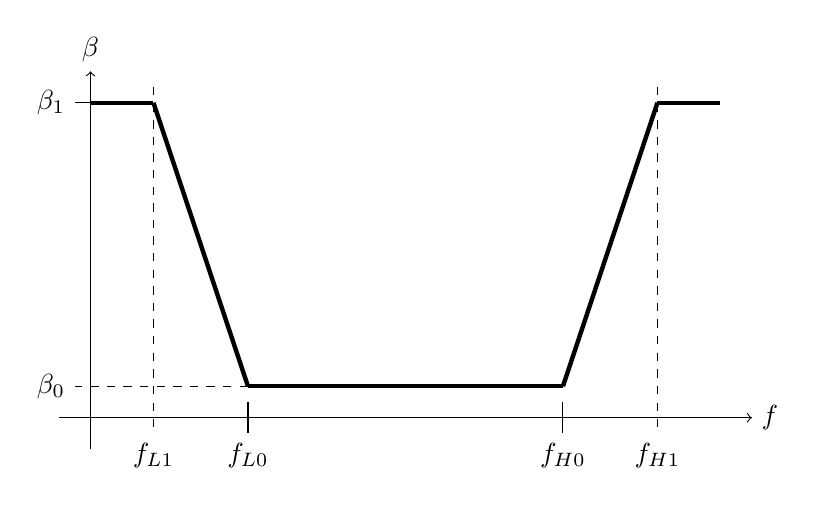
\begin{tikzpicture}[scale=4]
% Parameters
\def\betaone{1}; \def\betazero{0.1};
\def\fzero{0}; \def\fNyq{2};
\def\fLone{0.2}; \def\fLzero{0.5};
\def\fHzero{1.5}; \def\fHone{1.8};

% Axes
\draw[->] (\fzero-0.1,0) -- (\fNyq+0.1,0) node[right]{$f$};
\draw[->] (\fzero,-0.1) -- (\fzero,1.1) node[above]{$\beta$};

% Tick labels
\draw (\fzero+0.05,\betaone) -- (\fzero-0.05,\betaone) node[left]{$\beta_1$};
\draw[dashed] (\fLzero,\betazero) -- (\fzero-0.05,\betazero) node[left]{$\beta_0$};
\draw[dashed] (\fLone,\betaone+0.05) -- (\fLone,-0.05) node[below]{$f_{L1}$};
\draw (\fLzero,0.05) -- (\fLzero,-0.05) node[below]{$f_{L0}$};
\draw (\fHzero,0.05) -- (\fHzero,-0.05) node[below]{$f_{H0}$};
\draw[dashed] (\fHone,\betaone+0.05) -- (\fHone,-0.05) node[below]{$f_{H1}$};

% Plot
\draw[ultra thick] (\fzero,\betaone) -- (\fLone,\betaone);
\draw[ultra thick] (\fLone,\betaone) -- (\fLzero,\betazero);
\draw[ultra thick] (\fLzero,\betazero) -- (\fHzero,\betazero);
\draw[ultra thick] (\fHzero,\betazero) -- (\fHone,\betaone);
\draw[ultra thick] (\fHone,\betaone) -- (\fNyq,\betaone);
\end{tikzpicture}
\caption[Frequency-dependent regularization function for HRTF equalization.]{
Frequency-dependent regularization function of the inverse filters for HRTF equalization.}
\label{fig:A2_SABRE_Toolkit:Farina_Regularization}
\end{figure}

\paragraph*{Diffuse:} For headphones that employ diffuse-field equalization,
we can equalize the HRTFs by the average magnitude spectrum over all directions.
This is computed as the omnidirectional term of the spherical-harmonic decomposition of the HRTF magnitude spectra (in dB),
where the decomposition is computed using the pseudoinverse of $\mathbf{Y}$, given by~\eqnref{eq:YMatrix} for all measurement directions and up to order $L = 4$.
The equalization filter is then computed for the average magnitude spectrum using \eqnref{eq:A2_SABRE_Toolkit:EQ_Filter}.

\paragraph*{Horizontal:} Alternatively, we can compute an average HRTF over all horizontal-plane directions.
The procedure for this is very similar to the diffuse-field equalization, but the average spectrum is computed using only the HRTFs with elevation $|\theta| < 5^\circ$.
The equalization filter is then computed for the average magnitude spectrum using \eqnref{eq:A2_SABRE_Toolkit:EQ_Filter}.

\section{Summary}\label{sec:A2_SABRE_Toolkit:Summary}
The SOFA/ambiX binaural rendering (SABRE) toolkit described here is an open-source collection of MATLAB functions for generating custom binaural decoders.
The toolkit allows a user to construct, using any SOFA-formatted HRTFs, a custom binaural rendering configuration for the ambiX binaural plug-in.
Also implemented in the toolkit are several methods of HRTF interpolation, as well as common HRTF equalization options.
The toolkit is freely available online.\citefooturl{SABREToolkitURL}

\section*{Acknowledgements}
The SABRE toolkit relies on the ambiX ambisonic plug-in suite by \citet{Kronlachner2013,ambiXPlugInURL} and requires head-related transfer functions (HRTFs) stored in the SOFA format \citep{AES69-2015,SOFAMainPageURL}.
Accordingly, the SOFA API for MATLAB is needed to import the HRTF files (available online).\citefooturl{SOFAAPIURL}
The toolkit was originally presented by \citet{TylkaChoueiri2017b} at the 143\textsuperscript{rd} Convention of the Audio Engineering Society.